\chapter{Design}

In this chapter, we lay out the requirements for our implementation of Wasm containers in Apache OpenWhisk. Then we describe and discuss our implementation and the trade-offs involved.

\section{Requirements}

\subsection{Apache OpenWhisk}

In order to understand the requirements for our Wasm-flavored OpenWhisk, we need to understand the design of OpenWhisk itself first.

\begin{figure}
    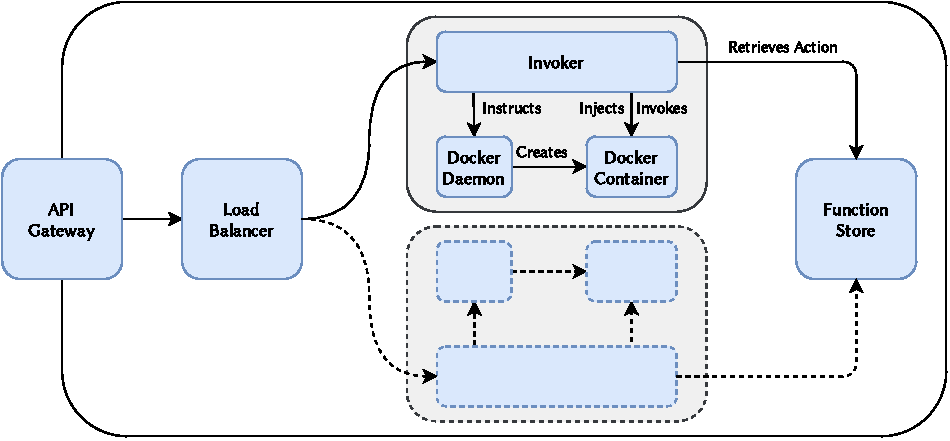
\includegraphics{figures/OpenWhiskActionInvocationFlow.pdf}
    \caption{Action invocation flow in Apache OpenWhisk based on the source code and documentation \cite{OpenWhiskSystemDesign}. Potentially many Invokers can exist in this setup.}
    \label{fig:openwhisk-action-invocation-flow}
\end{figure}

Figure \ref{fig:openwhisk-action-invocation-flow} sketches the design of OpenWhisk. Users interact with it through its API Gateway, which consists of \inl{nginx}, mostly for SSL termination, and the \inl{Controller}, which implements the main logic. It handles the creation of actions, OpenWhisk's name for serverless functions, authentication and authorization as well as invoking the action.
In the latter case, the controller uses its load balancer to determine which Invoker should handle the request, and publishes the request to an Apache Kafka queue, which the invoker is subscribed to. The controller and its load balancing take a central role in OpenWhisk, but in our figure it is represented by the API Gateway and the Load Balancer only, simply because we will not be modifying this part.
Our focus is on the Invoker. It is the part of OpenWhisk responsible for \emph{invoking} the action. A number of steps are involved in that process \cite{OpenWhiskSystemDesign}.

\begin{enumerate}
    \item It retrieves the action's code and execution permissions from an Apache CouchDB database, where the Controller stored it during action creation. 
    \item It instructs the local Docker daemon to start a new container, based on the runtime that the action needs to execute. This would be a \inl{openwhisk/action-nodejs-v10} image for JavaScript actions but could also be a generic black-box image (\inl{openwhisk/dockerskeleton}), that can execute any binary, such as one written in Rust or C.
    \item Finally, it injects the action's code into the container, invokes it with the given parameters and returns the result \cite{OpenWhiskSystemDesign}.
\end{enumerate}

Because OpenWhisk supports many runtimes and even the mentioned black-box image, it needs a common protocol to communicate with all of them. The just-described step 3 is the gist of that protocol. Each runtime needs to implement three endpoints. The \inl{/start} endpoint creates a new container and returns its address. The following requests to the \inl{/init} endpoint are then sent to that address, where the container receives the code and takes whatever steps necessary to make the action ready for execution. Thus, over a containers life cycle, this endpoint is called exactly once. Once initialized, the \inl{/run} endpoint can be called multiple times to execute the action \cite{OpenWhiskSystemDesign}.

That implies that the container isn't destroyed immediately after it has been invoked once. Indeed, OpenWhisk uses various optimizations of the described flow, in order to improve the system's performance. Among those are pre-warming containers or keeping the container running for some time after it has been invoked, before it is removed.
We will explore those optimizations in more depth later, to compare them to the optimizations in our Wasm runtime to better see where they coincide and differ \cite{OpenWhiskSystemDesign}.

% Describe deployment -- which of the components in the figure are packed as one in the deployment, i.e. in the kubernetes deployment with docker, the invoker and the containers are in the same pod

\subsection{OpenWhisk Modifications}

% Figure Planned modifications which is directly comparable to aboves figure

\begin{figure}
    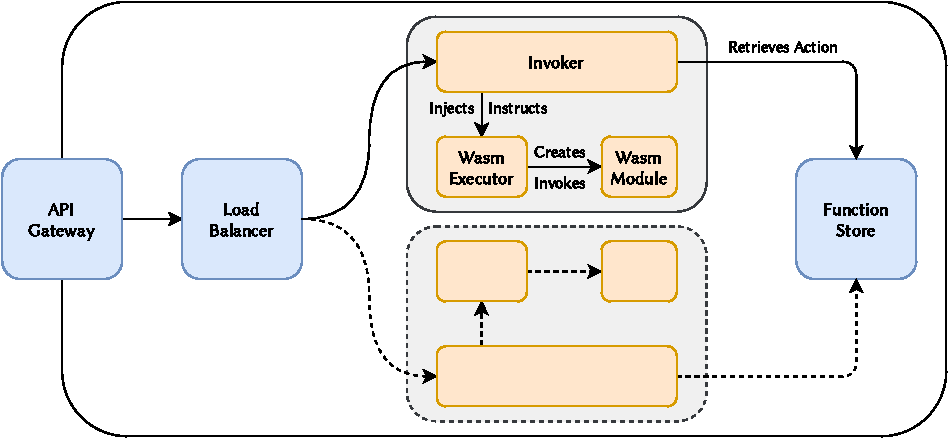
\includegraphics{figures/WasmOpenWhiskActionInvocationFlow.pdf}
    \caption{Invocation flow of a Wasm action in our modified Apache OpenWhisk.}
    \label{fig:wasm-openwhisk-action-invocation-flow}
\end{figure}

In this described invocation flow, we need to hook into OpenWhisk's invoker to enable its communication with the Wasm runtime we will implement, instead of the Docker daemon. Fortunately, the Invoker is already well-separated from the concrete containerization technology through a Service Provider Interface (SPI). OpenWhisk already supports Docker, but also Kubernetes as the container management system, such that the SPI was a logical addition. We implement a \inl{WasmContainer} that extends OpenWhisk's \inl{Container} abstraction, which already handles container communication, such as calling the \inl{/init} and \inl{/run} endpoints.

% Figure that shows a zoomed-in version of the invoker and its SPIs (as well as the Wasm runtime?) - Help better understand OW's design and what we added

In OpenWhisk's Docker container implementation, OpenWhisk only uses the Docker daemon to create a container, but then communicates with the container directly. In our implementation, every request is proxied through the \inl{WasmRuntime}. The advantage is, that not every Wasm module needs to implement the OpenWhisk protocol, which requires an HTTP server; increasing both the module's size and its runtime overhead. That presupposes, that the \inl{WasmRuntime} can handle a potentially large amount of requests.

% Need to decide whether OW handles containers life cycle or if runtime takes that responsibility

The runtime also needs to be fast in general, in order to aid in alleviating the cold start problem. That includes efficient handling of receiving the module's code from OpenWhisk, instantiating it and setting up the underlying Wasm executor. A general requirement for a useful Wasm runtime would also be its ability to run on different instruction set architectures.

In summary, the requirements for our runtime are

\begin{enumerate}
    \item It needs to be fast to alleviate the cold-start problem.
    \item It needs to run on devices with potentially different instruction set architectures.
    \item It needs to be able to efficiently handle a large amount of I/O concurrently, due to all requests being proxied through
\end{enumerate}

\section{Implementation}

To implement these requirements in Apache OpenWhisk we will take the following steps. The current Docker-based invoker will be replaced, to forward all the incoming requests to our new Wasm runtime.

The Wasm runtime will be written from scratch in the Rust programming language. There are a number of reasons for this choice.

\begin{itemize}
  \item It is a compiled language with performance close to that of C.
  \item It uses LLVM in the backend so that it can be compiled for almost any architecture.
  \item It allows for \quot{fearless concurrency}, since the compiler can detect data races at compile time.
  \item It has good support for asynchronous I/O, so it should be able to efficiently handle a large amount of concurrent requests.
  \item 3 out of the 4 Wasm executors investigated here are written in Rust, so embedding them is efficient and well documented.
\end{itemize}

The runtime consists of a web server that can take requests from the invoker asynchronously and concurrently. Because OpenWhisk doesn't communicate with the Wasm modules directly, but through the runtime, the \inl{/start} endpoint simply returns the runtimes own network address. This endpoint also returns an identifier for the container, so that OpenWhisk can handle its life cycle, i.e. the above-mentioned mechanism of keeping it warm for some time, for a faster subsequent invocation. There is a chance that this mechanism may not be necessary for Wasm modules, as they are much more lightweight in their instantiation. We will come back to this question later in our optimization discussion.

The entry point into our runtime will be through HTTP endpoints. In order for our runtime to handle requests concurrently, we use Rust's \inl{async} features. We will not make use of any advanced HTTP features, so the choice of the web framework doesn't matter too much. We use \inl{tide} \cite{Turon2021}, an asynchronous by-default web framework ideal for prototyping. It builds on top of \inl{async-std}, the asynchronous version of the Rust standard library.
Rust's async model works with \inl{Futures} -- also known as Promises in JavaScript -- which represent values that have not yet been computed. Contrary to \inl{Promises} however, Rust's \inl{Futures} are lazy: They do nothing unless actively polled. This task falls to \inl{async} runtimes, of which \inl{async-std} provides one. In \inl{async-std} the unit of execution is a \inl{Task}, which is similar to a \inl{Thread}, except it is driven to completion by the runtime instead of the OS. Many of those tasks are executed on the same thread, and by default, a \inl{Thread} per logical CPU core is spawned. Thus we have $M \cdot N$ tasks in total, where $M$ is the number of tasks per thread and $N$ the number of logical CPU cores.
From that, a second distinction is implied. A \inl{Task} should not do a blocking or long-running operation, like reading from a file via the standard library's \inl{std::fs::read_to_string}. Instead, it should use the \inl{async} version of that method, from \inl{async-std}, which does not block the thread. Otherwise, all other $M - 1$ tasks that are executed on the same thread will also be blocked, even though they may be able to progress. Note that, we could still process $N$ requests concurrently, even if tasks block, but that doesn't scale well enough. This is why async functions are also called cooperative routines (coroutines). When they need to wait for the OS to finish a task, they \emph{yield} to another routine.

As mentioned before, particularly long-running computations aren't a good fit for this execution model either. While one coroutine is computing, the others are -- once again -- waiting, similar to the blocking example. Executing a WebAssembly module is a long-running computation. Various data structures need to be created and the actual execution of the module is computationally intensive, since we embed the entire runtime.
To let the other coroutines make progress while we execute the module, we push the entire execution onto a thread pool. The coroutine then has the simple job of asynchronously waiting for that execution to finish and collecting the result. That allows the other coroutines to process more requests.

% Code-snippet task::spawn_blocking or similar


\subsection{Optimizations}

\begin{itemize}
    \item Caching of modules. What can be created per-thread different for each runtime (wasmtime, wasmer, ...)
    \item How important is the scale-to-zero principle vs. performance?
\end{itemize}